
\section*{练习}
\label{sec:ch01-exercises}

\begin{exercise}\label{ex:ch01-01}
设 $U$ 是 $\RR^n$ 的一个\trOpen{}子集，并设 $f\colon U\to\RR$ 是一个 $\cC^\infty$ 函数。设 $V$ 是 $\RR^n$ 的一个\trOpen{}子集，并设 $\varphi\colon V\to U$ 是一个\trDiffeomorphism。计算 $(d^2(f\circ\varphi))_y$（对 $y\in V$）。

设 $M$ 是一个\trManifold，并设 $g\colon M\to\RR$ 是一个函数。证明\trBilinearForm{} $(d^2g)_x$ 在向量子空间
\[
\operatorname{Ker}(dg)_x\subset T_xM\text{。}
\]
上是\trWellDefined{}的。\footnote{译注：此设问沿用\cref{thm:hessian-only-at-critical-points}的说法；\trHessian{}在 $\operatorname{Ker}(dg)$ 上的坐标无关性一般并不成立，参见该注记译注，此处不再重复。——译者注}
\end{exercise}

\begin{exercise}\label{ex:ch01-02}
\trManifold{} $V$ 的\trCotangent{}\trVectorBundle{} $T^*V$ 带有其自然的\trManifold{}结构（在附录~A 中回顾）。验证：我们可以把函数 $f\colon V\to\RR$ 的\trDifferential{} $df$ 看成\trCotangent{}\trVectorBundle{}的一个\trSection
\[
df\colon V\longrightarrow T^*V\text{，}
\]
亦即 $V$ 在 $T^*V$ 中的一个\trEmbedding。

在这种术语下，$f$ 的\trCriticalPoint{}是什么？证明：点 $a$ 是 $f$ 的一个\trNondegenerate\trCriticalPoint，当且仅当\trSubmanifold{} $df(V)$ 在所论的点处与\textbf{\trZeroSection}（zero section）\trTransverse。

证明函数的一个\trNondegenerate\trCriticalPoint{}必是\trIsolated{}的（不许用\trMorseLemma！）。
\end{exercise}

\begin{exercise}[猴\trSaddlePoint]\label{ex:ch01-03}
我们考虑函数
\[
\begin{array}{rcl}
f\colon \RR^2 & \longrightarrow & \RR\\
(x,y) & \longmapsto & x^3-3xy^2\text{。}
\end{array}
\]
考察\trCriticalPoint{} $(0,0)$。它是否\trNondegenerate{}？画出函数 $f$ 的几条\trRegular\trLevelSet，并画出它的图像。
\end{exercise}

\begin{exercise}\label{ex:ch01-04}
若 $f\colon V\to\RR$ 与 $g\colon W\to\RR$ 都是\trMorseFunction，那么 $f+g\colon V\times W\to\RR$ 也是\trMorseFunction，其\trCriticalPoint{}恰为 $f$ 与 $g$ 的\trCriticalPoint{}所成的点对。
\end{exercise}

\begin{exercise}[论复\trProjectiveSpace]\label{ex:ch01-05}
经作商，$\CC^{n+1}-\{0\}$ 上由
\[
f(z_0,\dotsc,z_n)=\frac{\displaystyle\sum_{j=0}^{n} j\,|z_j|^2}
                         {\displaystyle\sum_{j=0}^{n}|z_j|^2}
\]
定义的函数在复\trProjectiveSpace{} $\CP^n(\CC)$ 上诱导出一个函数，我们仍把它记作 $f$。

验证：这是一个\trMorseFunction，其\trCriticalPoint{}为诸点 $[1,0,\dotsc,0]$（\trIndex{}为 $0$）、$[0,1,0,\dotsc,0]$（\trIndex{}为 $2$），如此等等，直至 $[0,\dotsc,0,1]$（\trIndex{}为 $2n$）。
\end{exercise}

很想知道这个函数究竟从何而来的读者（当然出自 [54]——但在那之前呢？），可以去查阅\cref{thm:projective-perfect}。

\begin{exercise}[论\trSphere{}与实\trProjectivePlane]\label{ex:ch01-06}
用本质上相同的公式，现在考虑函数
\[
\begin{array}{rcl}
f\colon S^2 & \longrightarrow & \RR\\
(x,y,z) & \longmapsto & y^2+2z^2
\end{array}
\]
以及由它经作商而得的、实\trProjectivePlane{}上的函数 $g\colon \CP^2(\RR)\to\RR$。验证 $f$（从而 $g$）是一个\trMorseFunction，并证明它有六个\trCriticalPoint（从而 $g$ 有三个）：
\begin{itemize}
\item 两个\trIndex{}为 $0$ 的点，即点 $(\pm1,0,0)$，位于水平 $0$；
\item 两个\trIndex{}为 $1$ 的点，即点 $(0,\pm1,0)$，位于水平 $1$；
\item 两个\trIndex{}为 $2$ 的点，即点 $(0,0,\pm1)$，位于水平 $2$。
\end{itemize}
\cref{fig:morse-projective-plane}给出了该函数在\trSphere{}上的几条\trLevelSet。包含那两个\trIndex{}为 $1$ 的点的\trCriticalLevel{}集，由\trSphere{}与平面 $z=\pm x$ 相交而得的两个圆组成。
\end{exercise}

\begin{exercise}\label{ex:ch01-07}
在一个正方形中，画出“内胎”\trTorus{}上\trHeightFunction{}的诸\trLevelSet（答案就在本书的某处）。
\end{exercise}

\begin{exercise}[\trProjective\trQuadric]\label{ex:ch01-08}
我们考虑 $\CP^3(\CC)$ 中由方程
\[
z_0^2+z_1^2+z_2^2+z_3^2=0\text{。}
\]
定义的“\trQuadric” $Q$。证明：$Q$ 是\trManifold{} $\CP^3(\CC)$ 的一个（实）维数为 $4$ 的\trCompact\trSubmanifold。

我们记 $z_j=x_j+i y_j$（对 $0\le j\le 3$），而对 $z\in\CC^4$ 记 $z=x+i y$，其中 $x,y\in\RR^4$。我们取定两个实数 $\lambda$ 与 $\mu$，并对 $z\in\CC^4$ 令
\[
\widetilde{f}(z)=\lambda(x_0y_1-x_1y_0)+\mu(x_2y_3-x_3y_2)\text{。}
\]
验证：对 $|u|=1$，我们有
\[
\widetilde{f}(uz)=\widetilde{f}(z)\text{，}
\]
并由此推出 $\widetilde{f}$ 定义了一个函数
\[
\begin{array}{rcl}
f\colon \CP^3(\CC) & \longrightarrow & \RR\text{。}
\end{array}
\]
设出现在 $f$ 的定义中的实数 $\lambda$ 与 $\mu$ 满足 $0<\lambda<\mu$。令 $g$ 为 $f$ 在 $Q$ 上的限制。证明：$g$ 是一个\trMorseFunction，它有一个局部极小值、一个局部极大值以及两个\trIndex{}为 $2$ 的\trCriticalPoint。\footnote{译注：$\widetilde{f}$ 对 $z$ 是二次齐次的而非不变（$\widetilde{f}(2z)=4\widetilde{f}(z)$，$z$ 与 $2z$ 处的值相差 $4$ 倍），直接按非零代表取值并不\trWellDefined{}；应先限制到单位\trSphere{}（等价地取 $f([z])=\widetilde{f}(z)/\|z\|^{2}$）再降到 $\CP^3(\CC)$ 上。此处照原书排印，存疑备案。——译者注}
\end{exercise}

\begin{figure}[htbp]
  \centering
  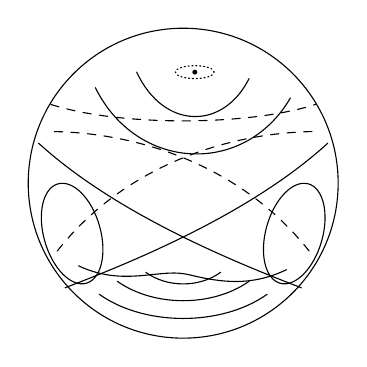
\begin{tikzpicture}[scale=0.82,line cap=round,line join=round]
    \draw (0,0) circle (2.4);%
    \fill (0.18,1.72) circle (1.1pt);
    \draw[densely dotted] (0.18,1.72) ellipse (0.30 and 0.10);
    \draw[dashed] (-2.05,1.22) .. controls (-1.0,0.88) and (1.0,0.88) .. (2.05,1.22);
    \draw (-0.72,1.72) .. controls (-0.30,0.82) and (0.62,0.82) .. (1.02,1.62);
    \draw (-1.36,1.48) .. controls (-0.72,0.18) and (0.95,0.10) .. (1.66,1.32);
    \draw (-2.24,0.62) .. controls (-1.1,-0.42) and (0.6,-1.15) .. (1.83,-1.62);
    \draw (2.24,0.62) .. controls (1.1,-0.42) and (-0.6,-1.15) .. (-1.83,-1.62);
    \draw[dashed] (-1.95,-1.05) .. controls (-0.9,0.28) and (0.7,0.78) .. (2.02,0.80);
    \draw[dashed] (1.95,-1.05) .. controls (0.9,0.28) and (-0.7,0.78) .. (-2.02,0.80);
    \draw[rotate around={16:(-1.72,-0.78)}] (-1.72,-0.78) ellipse (0.44 and 0.80);
    \draw[rotate around={-16:(1.72,-0.78)}] (1.72,-0.78) ellipse (0.44 and 0.80);
    \draw (-1.30,-1.72) .. controls (-0.6,-2.22) and (0.6,-2.22) .. (1.30,-1.72);
    \draw (-1.02,-1.52) .. controls (-0.45,-1.92) and (0.45,-1.92) .. (1.02,-1.52);
    \draw (-0.58,-1.38) .. controls (-0.25,-1.62) and (0.25,-1.62) .. (0.58,-1.38);
    \draw (-1.62,-1.28) .. controls (-0.9,-1.62) and (-0.35,-1.30) .. (0.10,-1.42)
          .. controls (0.60,-1.54) and (1.05,-1.60) .. (1.60,-1.34);
  \end{tikzpicture}
  \caption{实\trProjectivePlane{}上的一个\trMorseFunction}
  \label{fig:morse-projective-plane}
\end{figure}

\begin{exercise}\label{ex:ch01-09}
在本练习中，我们为“\trManifold{}上存在丰富的\trMorseFunction”提出另一种证明——更确切地说，即\cref{thm:morse-dense-open}的另一种证明：

\begin{enumerate}[label=(\arabic*)]
\item 利用（比如说）\cref{ex:ch01-02}，证明：\trCompact\trManifold{} $V$ 上\trMorseFunction{}的集合在 $\cC^2$ \trTopology{}下是\trOpen{}的，从而在 $\cC^\infty$ \trTopology{}下也是\trOpen{}的。
\item 设 $a\in V$，并设 $U$ 是某张以 $a$ 为中心的\trChart{}里的一个\trOpen{}集。我们以 $\mathcal{F}$ 表示定义在 $U$ 上的诸函数之\trDifferential{}全体（或者说，\trExact{} 1-\trForm{}全体）所成的空间，并将其视为 $\cC^\infty(U;(\RR^n)^*)$ 的一个子集（对每个 $x\in U$，$(df)_x$ 是 $\RR^n$ 上的一个线性泛函）。注意 $\mathcal{F}$ 并不是一个\trOpen{}子集。设 $\alpha$ 是一个\textbf{\trPlateauFunction}（plateau function），其\trSupport{}落在 $U$ 内，且在 $a$ 的一个\trCompact{}邻域 $K$ 上取值 $1$。对 $\varphi=df\in\mathcal{F}$，我们令
\[
\begin{array}{rcl}
F\colon U\times(\RR^n)^* & \longrightarrow & \RR\\
(x,A) & \longmapsto & f(x)+\alpha(x)A\cdot x\text{。}
\end{array}
\]
对 $x\in K$ 计算\footnote{若 $f$ 是一个依赖两个变量的函数 $(u,v)\in U\times V\subset E\times F$，则我们以 $(D_1f)_{(u,v)}$ 记线性映射 $(D_1f)_{(u,v)}\colon E\to\RR$，即 $f$ 关于第一个变量的偏\trDifferential；对于 $(D_2f)_{(u,v)}$ 亦有类似的记号。}$(D_1F)_{(x,A)}$，并证明映射 $D_1F$ 是一个\trSubmersion\footnote{译注：原书此句印作 “show that $F$ is a submersion”，漏印 $D_{1}$；按 $F$ 的值域为 $\RR$、且证明所用者为 $(D_1F)_{(x,A)}$ 对 $A$ 的线性性（映射 $(x,A)\mapsto D_1F(x,A)$ 对 $A$ 的\trDifferential{}为恒等），所证的\trSubmersion{}应是映射 $D_1F$；此处径改。——译者注}
\[
K\times(\RR^n)^*\longrightarrow(\RR^n)^*\text{。}
\]
证明 $\mathcal{F}$ 局部\trTransverse{}于 $\{0\}$（按\cref{subsec:transversality-theorems}中的意义）。
\item 证明 $V$ 的每一点 $a$ 都容许一个\trCompact{}邻域 $K$，使得在 $K$ 内的\trCriticalPoint{}皆为\trNondegenerate{}的那些函数 $f\colon V\to\RR$ 所成的集合，在 $\cC^\infty(V;\RR)$ 中是\trDense{}的。
\item 由此推演出\cref{thm:morse-dense-open}的一个证明。
\end{enumerate}
\end{exercise}
